\section{Experimental Results}
\label{sec:results}

\subsection{Experimental Setup}
\label{sec:res-setup}

All designs target the Ultra96-v2, a Zynq UltraScale+ ZU3EG device. Its
programmable logic provides 70{,}560 LUTs, 141{,}120 flip-flops, 360 DSP slices,
and 216 block-RAM tiles of 36\,Kb, with no UltraRAM; these bounds are the budget
against which we report utilization.

We evaluate on the 133-image test set. On imbalanced data, overall accuracy is an
incomplete summary: it is dominated by the larger classes and says nothing about
how errors distribute across them. We therefore report macro-averaged precision,
recall, and F1, and take macro F1 as the primary metric, since it averages the
classes with equal weight so that the minority classes count as much as the
majority. For the deployed models we also report weighted F1, to summarize the
test-set performance under the observed class frequencies, and add the per-class
precision, recall, and F1, which show how the errors distribute across the
classes. Macro values are bootstrap means over the test set, while accuracy and
weighted F1 are point values. 

\subsection{Knowledge Distillation}
\label{sec:res-kd}

Table~\ref{tab:kd} lists the full-precision macro-averaged metrics along the kept distillation
chain: the lesion-crop ResNet-50, the full-field ResNet-50 it teaches, the
ResNet-18 assistant, and the final student. The deployable \texttt{test\_resnet}
is small enough that distilling the full-field teacher into it directly triggers
the capacity-gap degradation of Section~\ref{sec:method-kd}. The intermediate
ResNet-18 assistant mitigates it: in a controlled comparison, distilling the
student through the assistant rather than straight from the teacher raises its
macro F1 by about nine points, the recovery the capacity-gap argument predicts
when teacher and student differ too much in size. Distilled through the assistant,
the student reaches 79.70 accuracy and 73.92 macro F1 at the $160\times160$
input.

\begin{table}[H]
\centering
\caption{The distillation chain.}
\label{tab:kd}
\begin{tabular}{lcccc}
\toprule
Model & Acc & Prec. & Rec. & F1 \\
\midrule
ResNet-50 (lesion-crops)   & 88.72 & 87.45 & 87.83 & 87.38 \\
ResNet-50 (full field)    & 92.48 & 94.22 & 89.68 & 91.39 \\
ResNet-18 (assistant)           & 90.98 & 91.20 & 88.41 & 89.30 \\
\texttt{test\_resnet} & 79.70 & 85.00 & 71.69 & 73.92 \\
\bottomrule
\end{tabular}
\end{table}

\subsection{Quantization and Bit-Width Exploration}
\label{sec:res-qat}

Table~\ref{tab:qat} lists the macro-averaged metrics of \texttt{test\_resnet} at
full precision and after QAT, with weights and activations quantized to the same
width. Both 8-bit and 6-bit QAT preserve the full-precision accuracy: each reaches
81.20 accuracy, above the 79.70 full-precision baseline. The 6-bit run is slightly
stronger on the macro metrics, reaching 76.39 macro F1 against 75.97 for 8 bits,
so reducing precision from 8 to 6 bits does not introduce an accuracy penalty in
software. At 4 bits training fails to recover, the validation macro F1 stalling
around 60.

\begin{table}[H]
\centering
\caption{Full-width quantization.}
\label{tab:qat}
\begin{tabular}{lcccc}
\toprule
Precision & Acc & Prec. & Rec. & F1 \\
\midrule
Full precision & 79.70 & 85.00 & 71.69 & 73.92 \\
8-bit          & 81.20 & 81.71 & 74.19 & 75.97 \\
6-bit          & 81.20 & 82.74 & 74.34 & 76.39 \\
\bottomrule
\end{tabular}
\end{table}

\subsection{Design Space Exploration}
\label{sec:res-dse}

For our network the binding resource is block RAM: logic and DSP slices stay
comfortably within budget, but on-chip memory does not, so fitting the accelerator
is a problem of block-RAM allocation. Following the mechanism described in
Section~\ref{sec:method-hw}, we map FIFOs below a depth threshold to LUTRAM and
leave deeper FIFOs in block RAM, where they use the primitives more efficiently.
This memory-style relief is the step that brings the design within the device:
without it the accelerator overruns the available block RAM at every precision,
and with it block-RAM utilization is the measure that separates the configurations
that fit from those that do not.

\begin{figure}[H]
\centering
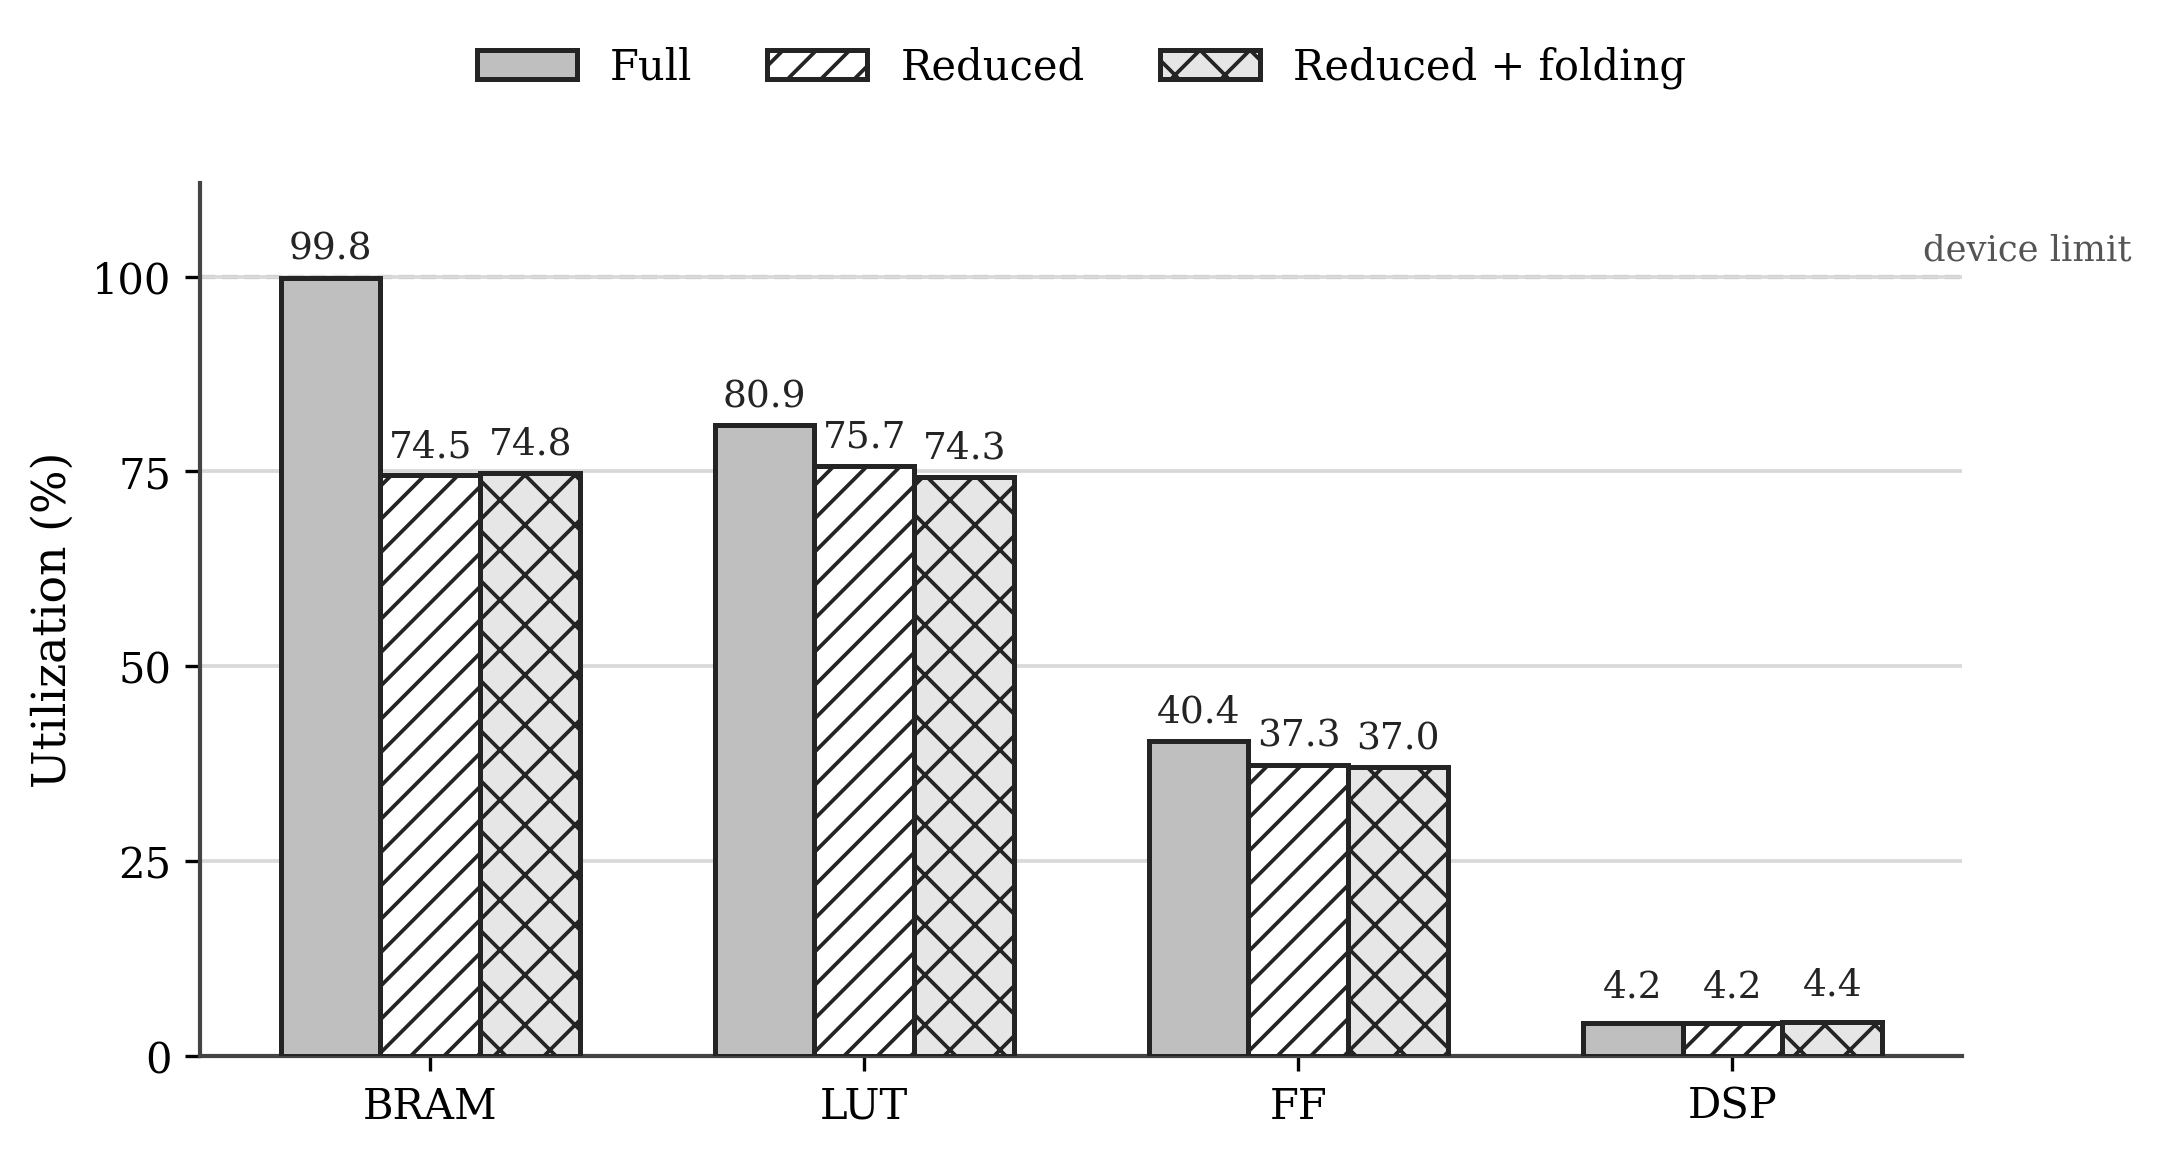
\includegraphics[width=\columnwidth]{figures/resource_utilization.png}
\caption{Resource projection.}
\label{fig:resource-util}
\end{figure}

With the relief applied throughout, the three precisions behave differently on the
full \texttt{test\_resnet}. At 8 bits the wider weights and activations overutilize
both block RAM and LUTRAM under the FINN configurations we evaluated, so that
precision is not deployable. At 6 bits the accelerator fits, with block RAM at
99.8\%, LUTs at 80.9\%, and flip-flops and DSPs far from full
(Figure~\ref{fig:resource-util}). At 4 bits accuracy has already collapsed
(Section~\ref{sec:res-qat}), so that precision is never built. Six bits is thus the
only setting that both fits the device and preserves accuracy, and is therefore
our first deployable design. This design uses the baseline FINN folding point for
the matrix-vector units, with PE and SIMD set to 1. Since block RAM
is already at 99.8\%, there is no practical headroom for increasing those factors.

\begin{table}[H]
\centering
\caption{Reduced-width quantization.}
\label{tab:slim}
\begin{tabular}{lcccc}
\toprule
Precision & Acc & Prec. & Rec. & F1 \\
\midrule
Full precision & 80.45 & 82.22 & 72.00 & 74.11 \\
8-bit          & 81.20 & 80.06 & 75.75 & 76.86 \\
6-bit          & 80.45 & 79.01 & 74.77 & 75.62 \\
\bottomrule
\end{tabular}
\end{table}

To trade a small accuracy margin for the headroom that more parallelism needs, we
introduce a narrowed variant, the \texttt{slim\_test\_resnet}, whose last two
channel widths are reduced from 192 and 96 to 128 and 64, then retrained under the
same distillation and QAT procedure. Table~\ref{tab:slim} reports its software
accuracy. At full precision it reaches 80.45 accuracy and 74.11 macro F1, 0.75
points of accuracy below the full network. The 8-bit QAT model reaches 81.20
accuracy and 76.86 macro F1. At 6 bits, the model holds 80.45 accuracy and 75.62
macro F1. As at full width, 4-bit training collapses and is discarded.

On hardware the reduced-width model repeats this bit-width pattern. At 8 bits it
still overutilizes block RAM and LUTRAM, as the full network does, so the most
accurate configuration again does not fit. At 6 bits it fits with room to spare: the
narrower stages reduce weight storage, bringing block RAM to about 74.5\% before
any extra folding. We do not prescribe a custom per-layer folding configuration;
instead, we raise FINN's target-FPS parameter until its automatic folding pass
selects the first additional parallelization step. This keeps block RAM at
74.8\%; more aggressive target-FPS values were also tested, but the FIFO depths
selected by FINN grew enough to overutilize block RAM again. LUTs and flip-flops slightly
decrease, while DSP use stays essentially unchanged except for the one additional
unit introduced by the folded reduced-width design
(Figure~\ref{fig:resource-util}). Six bits is therefore the precision we deploy,
now with the block-RAM headroom for useful parallelism that the full model lacked.
Figure~\ref{fig:resource-util} therefore reports three resource configurations:
the full-width graph, the reduced-width graph, and the reduced-width graph after
the selected extra folding.

\begin{table}[H]
\centering
\caption{Timing report.}
\label{tab:timing}
\footnotesize
\begin{tabular}{llrrr}
\toprule
Model & Build & Req. & Impl. & WNS \\
\midrule
Full    & unfolded & 100 & 100   & $+4.21$ \\
        & unfolded & 200 & 187.5 & $+0.30$ \\
\midrule
Reduced & unfolded & 100 & 100   & $+3.70$ \\
        & folded   & 100 & 100   & $+4.13$ \\
        & folded   & 200 & 187.5 & $+0.19$ \\
\bottomrule
\end{tabular}
\end{table}

Every build in Table~\ref{tab:timing} meets timing at its implemented clock; the
requested and implemented clocks are in MHz and WNS is in ns. The full network
closes without extra folding at 100\,MHz with 4.21\,ns of slack and at
187.5\,MHz with 0.30\,ns of slack. The reduced-width network first closes without
extra folding at 100\,MHz with 3.70\,ns of slack. After the selected folding step,
it still closes at 100\,MHz, with 4.13\,ns of slack, and reaches 187.5\,MHz with
0.19\,ns of slack when the clock target is tightened. We therefore use
187.5\,MHz as the deployed clock: it is the fastest frequency reached by the flow
with positive slack and is already close to the timing limit.

\subsection{Hardware Deployment Results}
\label{sec:res-hw}

The design-space exploration leaves two deployable 6-bit accelerator families on
the Ultra96: the full-width \texttt{test\_resnet}, which gives the highest board
accuracy, and the reduced-width variant, which sacrifices a small accuracy margin
for the memory headroom needed by folding. Clock and folding do not change the
quantized weights or the predicted labels, so classification performance is
reported once per family. In both cases the deployed hardware is bit-exact with
its software reference on the 133-image test payload.

\begin{table}[H]
\centering
\caption{Deployment accuracy.}
\label{tab:deployment}
\begin{tabular}{lrrr}
\toprule
Family & Acc & wF1 & mF1 \\
\midrule
Full    & 81.20 & 80.39 & 76.77 \\
Reduced & 80.45 & 79.89 & 75.62 \\
\bottomrule
\end{tabular}
\end{table}

Table~\ref{tab:deployment} gives the on-board accuracy view. The full-width
family reaches 81.20 accuracy and 76.77 macro F1, while the reduced-width family
reaches 80.45 accuracy and 75.62 macro F1. The cost of the reduced-width design
is therefore 0.75 percentage points of accuracy, with almost no movement in
weighted F1. The per-class breakdown in Table~\ref{tab:per-class} shows where
that residual error lies.

\begin{table}[H]
\centering
\caption{Per-class deployment metrics.}
\label{tab:per-class}
\begin{tabular}{llrrrr}
\toprule
Family & Class & n & Prec. & Rec. & F1 \\
\midrule
Full & Healthy  & 47 & 78.3  & 100.0 & 87.8 \\
     & Nevus    & 44 & 80.0  & 81.8  & 80.7 \\
     & Melanoma & 26 & 100.0 & 65.4  & 78.7 \\
     & CHRPE    & 16 & 72.6  & 50.2  & 58.4 \\
\midrule
Reduced & Healthy  & 47 & 82.5 & 100.0 & 90.3 \\
     & Nevus    & 44 & 79.1 & 77.3  & 78.0 \\
     & Melanoma & 26 & 94.5 & 65.5  & 77.0 \\
     & CHRPE    & 16 & 60.0 & 56.3  & 57.2 \\
\bottomrule
\end{tabular}
\end{table}

Neither family collapses on any class. Both recover every healthy image, and
nevus remains balanced between precision and recall. The clinically harder
minority classes carry most of the residual error. Melanoma precision stays high
in both families, but recall remains close to 65\%, so missed malignancies are
the main clinical weakness. CHRPE is the weakest class by F1 in both families,
consistent with its small support and its visual overlap with nevus.

The throughput results show the effect of the freed memory on folding. The
full-width family keeps the baseline FINN folding point and reaches
3.39 images/s at 100\,MHz and 6.36 images/s at the routed 187.5\,MHz clock. The
reduced-width family is first measured without extra folding at 100\,MHz, where
it matches the same 3.39 images/s baseline. After the automatic folding step
selected in Section~\ref{sec:res-dse}, it reaches 6.78 images/s at 100\,MHz and
12.71 images/s at 187.5\,MHz (Figure~\ref{fig:deployment-throughput}).

\begin{figure}[H]
\centering
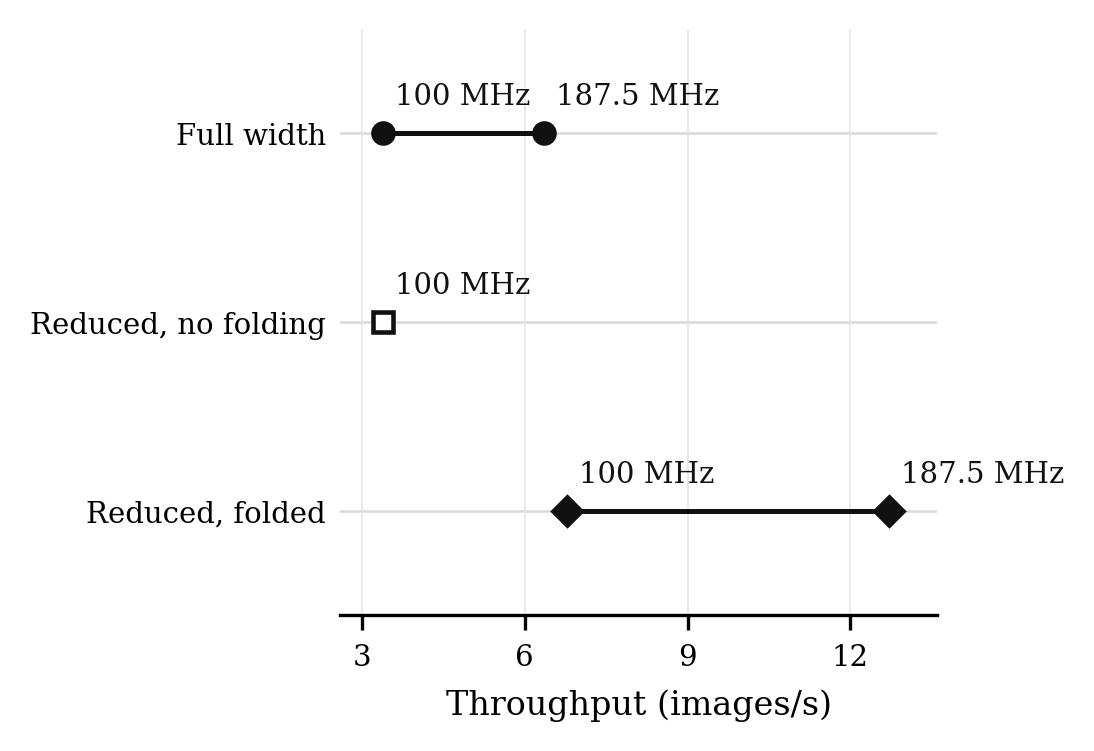
\includegraphics[width=\columnwidth]{figures/deployment_tradeoff.png}
\caption{Throughput operating points.}
\label{fig:deployment-throughput}
\end{figure}

The gain at the fastest clock is therefore not a clock-only effect: both families
are evaluated at 187.5\,MHz, but the reduced-width graph has enough memory margin
for the extra folding step. This raises throughput from 6.36 to 12.71 images/s at
the same clock, at the 0.75-point accuracy cost reported above.
